\documentclass[a4paper,11pt]{article}
\usepackage{graphicx}
\usepackage{amsmath}
\usepackage{lscape}
\usepackage{capt-of}
\usepackage{lmodern,textcomp}
\usepackage{fancyhdr}
\usepackage{caption}
\usepackage{mathtools}
\usepackage{subcaption}
\usepackage{url}
\usepackage{footnote}
\usepackage{tikz}
\usetikzlibrary{arrows.meta}
\usepackage{enumerate}
\usepackage{listings}
\usepackage{siunitx}
\usepackage{float}
\usepackage{eurosym}
%external reference to pick references from pictures.tex. 
%Note: This is does not bring the content of pictues.tex but for only ref. To import content use \input.
\usepackage{xr}
\externaldocument{pictues.tex}

\usetikzlibrary{quotes,angles,positioning}
\usepackage{standalone}
\usepackage{multirow}
\usepackage{geometry} % to change the page dimensions
\geometry{a4paper} 
\pagestyle{fancy}
\lhead{}
\rhead{Louis Carnec \\ Vijay Katta \\ Adedayo Adelowokan}
\renewcommand{\headrulewidth}{0pt}
\setlength\parindent{0pt}
\usepackage{amstext} % for \text
\DeclareRobustCommand{\officialeuro}{%
  \ifmmode\expandafter\text\fi
  {\fontencoding{U}\fontfamily{eurosym}\selectfont e}}
\begin{document}



\begin{titlepage}

\newcommand{\HRule}{\rule{\linewidth}{0.5mm}} % Defines a new command for the horizontal lines, change thickness here

\center % Center everything on the page
 

%----------------------------------------------------------------------------------------
%	TITLE SECTION
%----------------------------------------------------------------------------------------

\HRule \\[0.4cm]
{ \huge \bfseries Analytical Business Modelling Assignment 3}\\[0.4cm] % Title of your document
\HRule \\[1.5cm]
 
%----------------------------------------------------------------------------------------
%	AUTHOR SECTION
%----------------------------------------------------------------------------------------

\begin{minipage}{0.4\textwidth}
\begin{flushleft} \large
\emph{Students:}\\
Louis \textsc{Carnec}\\ % Your name
Vijay \textsc{Katta}\\ % Your name
Adedayo \textsc{Adelowokan}
\end{flushleft}
\end{minipage}
~
\begin{minipage}{0.4\textwidth}
\begin{flushright} \large
\emph{Student \#:} \\
15204934\\ % Supervisor's Name
15202724\\
15204151
\end{flushright}
\end{minipage}\\[4cm]

% If you don't want a supervisor, uncomment the two lines below and remove the section above
%\Large \emph{Author:}\\
%John \textsc{Smith}\\[3cm] % Your name

%----------------------------------------------------------------------------------------
%	DATE SECTION
%----------------------------------------------------------------------------------------

{\large \today}\\[3cm] % Date, change the \today to a set date if you want to be precise

%----------------------------------------------------------------------------------------
%	LOGO SECTION
%----------------------------------------------------------------------------------------

%\includegraphics{Logo}\\[1cm] % Include a department/university logo - this will require the graphicx package
 
%----------------------------------------------------------------------------------------

\vfill % Fill the rest of the page with whitespace

\end{titlepage}

\section{Introduction}
%DAYO{
In the real-world companies are faced with problems regarding the transportation of goods, people or information. A couple of important challenges companies are faced with are finding ways to increase profits, reduce costs and further increase customer satisfaction. One of the many ways companies can save costs is in having an effective supply chain management which involves choosing distribution center locations or improving their delivery system. 

The choice of locations can reduce transportation costs, and reduce lead times. By reducing lead times, inventory control becomes easier which in turn increases service level \cite{gallmann2011linking}. The factors for choosing a location go beyond lead time and reduction of costs, factors like the surrounding community also have a significant effect. For example, the strength of the infrastructure (road etc.) surrounding the location, reliability, congestion and vulnerability. An area with a strong infrastructure that is further away could be more beneficial to an area that is closer with weak infrastructure. These are the type of factors that could affect the supply chain, in service level, costs etc. 

Improving the delivery system would also bring the same benefits as choosing the right location for a depot. In this case, a company would need a Vehicle Routing Problem (VRP) solution. VRP dates to the late 50s, although there has been nearly 60 years of research in this phenomenon large-scale versions of this problem still poses a challenge for the scientific community. 

Vehicle Routing Problem tries to find a way to visit several locations given a certain number of vehicles in a cost-effective way. The simplest definition states that every customer is visited by one vehicle, and each vehicle does one trip starting and ending at the depot. The question now is what order should customers be visited while ensuring that the various constraints are considered. This is the problem we will be addressing in this assignment.
%}

\section{Application: Goods Delivery}
%LOUIS{
The case study problem we have tackled is the delivery of goods throughout Irish cities and towns from a single depot location based in Dublin given a general time window constraint on delivery times. A single vehicle, with a given carrying capacity, must deliver goods to all towns/nodes in the graph and meet each town's demand for goods, that is deliver an amount of goods equal to that city's demand. Given the fact that each vehicle has a given capacity, the transportation vehicle can only take so many goods and must therefore revert back to the depot to pick up more goods to deliver. Further, deliveries must be conducted within a maximum number of working hours and the vehicle must return to the depot. Therefore, each `trip', if forced by the time constraint on working hours available, is a working day. Here a `trip' is a succession of edges connecting nodes that leaves and returns to the depot once. 

Our problem involves finding the optimal route for the vehicle so that costs are minimised, where costs incurred stem from the the time spent travelling across the route, the sum of the `trips'. This is a Vehicle Routing Problem (VRP), a variant of the Travelling Salesman Problem for which the \textit{order} of nodes in a graph to be visited must be optimised to find the tour with lowest travelled distance. 

In his chapter on vehicle routing, Cordeau warns that due to high variability of problems in practice, the objective function and constraints of VRP are highly variable and thus must be tailored to each problem \cite{cordeau2007vehicle}.
\\\\
We initially attempted to solve a slightly different version of the problem solved here and modelled in Section 3; the `Capacitated Vehicle Routing Problem' \cite{toth2002models}. In this problem multiple vehicles are used at the same time to deliver goods around the symmetric undirected graph. In our implementation we followed closely the implementation used in section 11.5 of  `Applications of optimization with Xpress-MP'  \cite{gueret1999applications} for planning flights. The model is similar to the one presented in this report, distance is minimised given that each node/city must only be visited once. To account for the fact that $n$ trips can be made by $n$ vehicles, an additional constraint is added to stipulate that the depot must have $n$ incoming edges. Optimising the model, we were able to create the subtours for the graph to be `broken' into $n$ subtours. Having Dublin as the depot, the $n$ closest cities to Dublin were used as outgoing/incoming nodes to be attached to the $n$ subtours. When it came to making subtour eliminiation procedure into $n$ subtours, we were unable to create a function which would allow us to form the subtour containing the depot to then break the smaller subtours.
%}



\section{Related Work}
%DAYO{
Combinatorial optimization problems have been studied in huge detail, the Vehicle Routing Problem was initially introduced in 1959 \cite{dantzig1959truck}. The needs of the transportation industry were the motivation behind the problem, especially realizing the amount of savings that could be made with small improvements in efficiency. Routing problems always have an abundance of complex constraints and variables, this is evident in the industry and our personal lives. These include traffic conditions, weather in certain situations, road-work etc. There are further constraints that would be specific to the industry which include shift limits for drivers, specified arrival and delivery times. The widely-studied version of VRPs are more simplistic, and utilize less constraints. The simpler versions still pose as a difficult task which shows how difficult it is to solve VRPs. 


\subsection{Travelling Salesman Problem}
The Travelling Salesman Problem (TSP) is one of the oldest known routing problems. It presents a salesman that has a specified number of cities to visit and needs to know the optimal order to visit these cities to minimize the distance needed to travel. TSP is an NP-hard problem \cite{lenstra1981complexity}.

\subsection{Vehicle Routing Problem}
VRP is also an NP-hard problem but it is safe to assume that the it iss a much harder problem to solve over TSP. VRP can be applied to various fields; logistics, communications, manufacturing, transportation, to list a few. In a VRP there are several vehicles that need to visit many customers. Vehicles starts at depot before visiting a section of the customers before returning to the starting depot. 
Capacitated Vehicle Routing Problem (CVRP) is a classic problem, this involves finding a solution to a transport problem where customers can be reached via multiple identical vehicles with different capacity restrictions. 
A special case of VRP is Vehicle Routing Problem with Time Windows (VRPTW). VRPTW comes with its own added complexity, each customer has a start and end time which indicates the time the vehicle should be servicing. An example of this application would be in case of a company that delivers heating oil. Although this constraint is hard, the vehicle does not need to arrive between that time, it can arrive before the start time but must remain inactive for a given period. 
Like TSP, VRP is an NP-hard problem \cite{lenstra1981complexity} but it safe to assume that the VRP is a much harder problem to solve than TSP. 
%}



%LOUIS{
\section{Mathematical Programming Model Formulation}

The formulation proposed in this report is an extension of the formulation proposed in the `Applications of optimization with Xpress-MP' book in section 10.4 \cite{gueret1999applications}. The formulation is extended by; adding a general time window which applies to all cities within the graph (as opposed to individualised time windows) and thus a constraint forcing the vehicle to return to the depot within the time window, an additional constraint to specify the number of times the vehicle can return to the depot and an probability parameter simulating the random probability of being stuck in traffic on a given leg of the trip.

\subsection{Assumptions}
Several assumptions are made in modelling this VRP problem.

We assume that the time taken to travel from one city to another is linearly proportional to the distance by air between the two points, as such in the mathematical formulation of the model distance, rather than time is minimised. It is also assumed that no time is lost at each node, that is the time taken for the route is equal to the time taken proportional to the distance. However, a fixed cost is incurred at each stop. This assumption means that for a route of length x, the time taken is the same whether there were 5 stops or 10 stops along the route. It is assumed that the distance covered over time does not affect cost. Cost is only related to time spent travelling, plus a fixed cost.


\subsection{Objective Function}

The objective function (\ref{eq1}) we wish to minimise is the cost of delivering goods throughout the graph.
\begin{equation}\label{eq1}
\textrm{Minimise}\quad  Cost = \quad \sum\limits_{i \in cities} \sum\limits_{j \in cities, i \neq j} c_{i,j}p_{i,j}
\end{equation}
Where, $$c_{i,j} = (d_{i,j}/kmph_{i,j})*cph + \bar{c}$$
$c_{i,j}$ is the cost of travelling from node $i$ to node $j$, which is given by the time taken to travel from $i$ to $j$ (distance / speed) times the cost per hour $cph$ for the given leg journey, plus a fixed cost for each stop $\bar{c}$. 
\\\\
There are three decision variables in this model, $p_{i,j}$ which states whether node $j$ is a successor to node $i$, the total quantity at node $i$ ($q_{i}$), and the total time spent delivering at node $i$ ($t_{i}$).

\begin{equation}\label{eq4}
p_{i,j} \in{\{0,1\}} \quad , \forall i,j \in cities\quad, where \quad i \neq j
\end{equation}

$p_{i,j}$ in (\ref{eq4}) is a binary decision variable which states that the vehicle travels from node $i$ to node $j$ if $p_{i,j}=1$. The total quantity delivered at $i$ ensures that the quantity delivered is equal to demand for each node and that each trip in the tour is conducted while respecting the maximal capacity of the vehicle. The total time delivering decision variable is similar to the total quantity delivered variable and ensures that the route respects the fact that there is a general time window to be respected for delivery and that the vehicle must return to the depot within this time window. By solving for these variable, the model should return the shortest route which respect to the constraints presented below.

\subsection{Constraints}

Equations (\ref{eq2}) and (\ref{eq3}) state that each city (expect from the depot, which is always node 1) must be entered and departed exactly once, so that every city is delivered to but that the tour is not unnecessarily extended by visiting nodes which have already been visited. Note that $i,j\neq1$ due to the fact that the depot can be entered and departed multiple times. The vehicle should return to the depot once it has delivered all goods within its capacity ($C$) or worked for a given number of hours ($H$, see Table 1). 

\begin{equation}\label{eq2}
\sum\limits_{i \in cities} p_{i,j} = 1 \quad , \forall j \in cities \quad, j\neq1
\end{equation}

\begin{equation}\label{eq3}
\sum\limits_{j \in cities} p_{i,j} = 1 \quad , \forall i \in cities\quad, i\neq1
\end{equation}



\subsubsection{Increasing Total Quantity}

The following constraints are used in finding the optimal tour given a set of constraints while solving for the decision variable total quantity, the total quantity delivered at a given node. The total quantity delivered at a given node ($q_{i}$) must be less or equal to the maximal capacity ($C$) of the delivering vehicle (\ref{Qleq}) and less or equal to the demand ($D_{i}$) / or the amount to be delivered at that node (\ref{Qgeq}). Constraint (\ref{Qleq}) forces the vehicle to take trips back to the depot if it must deliver a total demand greater then the total capacity of the vehicle.

Since total quantity delivered is a decision variable to be maximised within maximal capacity of the vehicle, constraint (\ref{Q}) ensures that the total quantity delivered if city $i$ is the first city visited \textit{in the trip} is equal to the demand at $i$, otherwise if $i$ is not the first city delivered to, then the total quantity at $i$ must be less or equal to the maximal capacity of the vehicle (while is already stated in (\ref{Qleq})). That is (\ref{Q}), resets the total quantity variable at each trip to the demand of the first node visited within a new trip. 

Constraint (\ref{incQ}) is a strictly increasing total quantity constraint. It states that if node $j$ follows node $i$, the total quantity delivered at $j$ must be the total quantity delivered at $i$ plus the demand at $j$. This constraint ensures that at each node successor node the total quantity delivered increases and that each `trip' is optimised.

\begin{equation}\label{Q}
q_{i} \leq C + (D_{i} - C) \times  p _{1,i} \quad, \forall i \in cities\quad, i\neq1
\end{equation}

\begin{equation}\label{incQ}
q_{j} \geq q_{i} + D_{i} - C + C*p_{i,j}  + (C-D_{j}-D_{i})*p_{j,i}\quad, \forall i \in cities\quad, i,j \neq 1 \quad, i\neq j
\end{equation}

\begin{equation}\label{Qleq}
q_{i} <= C \quad, \forall i\quad, i\neq1
\end{equation}

\begin{equation}\label{Qgeq}
q_{i} >= D_{i} \quad, \forall i\quad, i\neq1
\end{equation}


\subsubsection{Increasing Total Time Constraint}

The concept behind the total time of delivery constraints (\ref{T}), (\ref{incT}) and (\ref{leqT})  is the same as that of the (\ref{Q}) and (\ref{incQ}) constraints for total quantity delivered. (\ref{T}) ensures that the total time delivering at $i$, if $i$ is a successor to the depot (node 1), is equal to the time taken to deliver to that node. Alternatively if $i$ is not a successor to the depot node, the total time of delivery at $i$ is less or equal to the hours available for delivering in a day. Constraint (\ref{leqT}) is therefore made redundant in this case. Both constraints ensure that the vehicle returns to the depot within the delivering time limit allocated (before the end of the working day). The strictly increasing delivering time constraint (\ref{incT}) ensures that the total time of delivery at $j$ is equal to the total time of delivery at $j$, plus the time taken to travel from $i$ to $j$.

\begin{equation}\label{T}
T_{i} \leq H + (t_{1,i} - H) \times  p _{1,i} \quad, \forall i \in cities \quad, i\neq1
\end{equation}

\begin{equation}\label{incT}
T_{j} \geq T_{i} + t_{i,j} - H + H*p_{i,j}  + (H -  t_{i,j})p_{i,j} \quad, \forall i \in cities\quad, i,j \neq 1 \quad, i\neq j
\end{equation}

\begin{equation}\label{leqT}
q_{i} <= H \quad, \forall i\quad, i\neq1
\end{equation}


\subsubsection{Number of times through the depot}
Lastly, we present an optional constraint which forces the model to return a route solution with a given number of trips, or returns to the depot.

\begin{equation}\label{eq13}
\sum\limits_{i \in cities} p_{i,1} = n
\end{equation}

\begin{table}[h!]
\centering
\caption{List of Variables}
\label{variables}
\begin{tabular}{lll}
\hline
Decision Variables & Symbol & Description \\
\hline
\hline
Precedes & $p_{i,j}$  & Binary Variable - 1 if $i$ precedes $j$\\
Total Quantity & $q_{i}$ & Total Quantity Delivered at $j$ \\
Total Time & $T_{i}$ & Total Time Delivering at $j$ \\ 
\\
\hline
Variables & Symbol & Description \\
\hline
\hline
Distance & $d_{i,j}$ & Distance from $i$ to $j$  \\
Speed & $kmph_{i,j}$ & Average Constant Speed of Vehicle from $i$ to $j$\\
Cost per hour & $cph$ & Cost per hour of delivering \\ 
Fixed cost & $\bar{c}$ & Fixed Cost per stop \\
Capacity & C & Capacity of vehicle \\ 
Demand & $D_{i}$ & Demand / Quantity ordered at city $i$ \\  
Hours & $H$ & Maximal Delivering Hours \\
Travel Time & $t_{i,j}$ & Travel time from $i$ to $j$ \\ 
Trips & $n$ & Number of Trips \\
\end{tabular}
\end{table}

\section{Mosel Model}

The Mosel model used in this report is an application of the mathematical model presented above. It was run using both real and generated data. A probabilistic component was added to the travel between nodes/cities.

The city location and population data used to create the symmetric undirected graph of Irish cities was obtained from Tageo\footnote{\url{http://www.tageo.com/index-e-ei-cities-IE.htm}}. The data was cleaned in \texttt{python} and an adjacency matrix of the distance `by flight' between cities was calculated using the \textit{vincenty}\footnote{\url{https://geopy.readthedocs.io/en/1.10.0/}} distance (great-circle distance) from the \texttt{geopy} library.

Demand for each city was calculated within \texttt{Xpress Mosel} as being proportional to the population of each city with an added random component. 

To model the fact that travel time between two cities may be affected by traffic, we added a function which would assign different average speeds to different legs of the route. A node was given an 20\% chance of having an average speed of 60km/h and an 80\% chance of having a 100km/h average speed.

A printing procedure was created which would output the total distance covered, quantity delivered and number of stop for each `trip'.




\subsection{The model development process; what facilities/ features does the development environment
have to aid model development and solution of your problem? }

Xpress Mosel, the development environment used in conducting this report, allowed us, the users, to easily check the status of our model which was beneficial in developing and finding a solution to our model. 

The info bar, when an error occurs, outputs a range of errors in the code, this allowed us to quickly and easily debug our code. By right clicking on a variable within the text and showing values assigned to the variable, we were able to quickly check that each variable was correctly assigned, this was useful when working with a dummy data while building the model.
The `Run Bar' feature, to the right of the screen allowed us to check the solutions being produced when running the model by navigating to the `Solutions' tab. The `Stats' tab enabled us to check the status of the program without having to print it out. Finally the `Row View' feature within the `Matrix' tab allowed to test the effect of different vehicle capacity and time capacity parameters on the slack variables for each constraint.


\subsection{How easy is it to verify correctness of the model and to separate the problem and its data}
Verifying the correctness of the model was relatively simple. We built the model in \texttt{Xpress Mosel} using a dummy dataset containing a 5-by-5 adjacency matrix. Examining the solutions in `solution' tab within Xpress, we were able to verify that each of the model's constraints were being respected and that indeed for the small dummy dataset the result of the minimised objective function was as expected.

 Applying the Mosel model to our application of choice, after initialising the datafile containing the adjacency matrix for the distances of Irish cities, although the model itself remained the same, some of the model's parameters had to be altered to fit the new data in order for the model to output a result, otherwise the model would keep running. Constraints (\ref{Q}, \ref{incQ}, \ref{T} and \ref{incT}), depend on the capacity parameter and on the time available parameter of the vehicle. For some values of these parameters with a given dataset, the model will be infeasible. Additionally, the optional constraint for the number of times the vehicle must pass by the depot must be feasible. For example, if demand at city 1 is 400 units and the capacity of the vehicle is 300 units, the problem will be infeasible and Mosel will not find a solution. The capacity of the vehicle needs to be increased for the model to function. Likewise, if the speed of the vehicle is 20 km/h, the working hours of delivery are of 8 hours, the maximum distance covered in the route is 160 km.
 
In order to make the program more versatile in implementing with different datasets, we would have like to have created if-loops which would raise an error in case the parameters provided do not allow for a feasible solution to be found. If the program did not stop, this was generally due to a parameter making the problem infeasible. In this case we had to use the `Row View' tab within the environment to inspect each constraint in order to debug the program.

This versatility enables us to solve different problems. For example, we could solve a VRP, for picking up broken Dublin City Bikes from the various stations around Dublin. We would download the locations of the stations, create an adjacency matrix using the same \texttt{python} program used in creating the Irish cities adjacency matrix and solve for the quickest route. 

\subsection{How easy is it to either perform sensitivity analysis on the defined problem or to
amend/extend the problem? }

Amending and/or extending the problem presented here is feasible depending on the changes/extensions the user seeks to make. We have demonstrated that the model can be extended easily, by stipulating some additional constraints such as the number of times the vehicle must return to the depot and respecting time windows are easy. This is possible by altering/adding some constraints. 

Further, the model's parameters can easily be altered; such as the maximal capacity of the vehicle, the number of hours in the working day, the average speed of the vehicle, the probability of the time to go from one node to another increasing or decreasing.

However, for some changes/extensions, we would need a different model. If we wanted to change the model to use a number of $n$ vehicles to find $n$ tour for each vehicle so that each city is visited once, we would need to change the subtour elimination constraint completely. 

Further, if we were to extend the model to a case study with many more nodes, we would need to adopt a different formulation such as tree search or a heuristic approach \cite{gueret1999applications}. The model we are currently using would work for instances of up to 30 nodes only. Therefore, the Dublin Bikes case study proposed ion the previous section would be infeasible as there are 102 stations.



\subsection{What theoretical principles are demonstrated in your application?}

The theoretical principles demonstrated in our application come from \textit{network optimisation} and \textit{stochastic optimization}. The distance between cities, produced in the form of an adjacency matrix, represent a graph of cities where the nodes are cities and edge weights are the distances between them. Using combinatorial optimisation, the optimal set of nodes in a specific order are returned while respecting a set of constraints. At the same time this application is a stochastic optimisation problem as there is the presence of randomness in both the demand and speed variables, that is the result of the optimisation, the total cost of the route, should vary across runs of the model as it is affected by randomness. Using a stochastic optimisation model of this type allows us to more realistically \textit{simulate} the cost of a route. Running the model a number of times and getting a set of statistics which represent the results would enable us, the analysts, in making recommendations on best route to choose to minimise cost.

%}
\section{Results}

We ran the \texttt{Xpress Mosel} model  to find the optimal vehicle route on datasets of different size - 5,  20 and 30 cities, for two different scenarios -1) With Capacity Constraint and No Time Constraint and 2) With Capacity and Time Constraint. The distance between any two cities remains same in either direction, but the speed of the vehicle can be different and the model takes this into consideration while finding the minimal cost route. First line of the output is the total transportation cost of the goods delivered in all the trips from the warehouse. Second line has five different columns - route of journey (from city -to city), distance between the cities in kilo meters , speed in kilo meters per hour, time in hours and finally quantity of goods delivered. Other statics such as quantity 
delivered, distance covered and number of stops are for a given a trip from the central warehouse in Dublin. Executing each instance of 5 cities and 20 cities took less than a second and 30 cities took about 5 seconds. It is possible that the run time increases exponentially as the number of cities increases but for all practical purposes of delivering the goods the model works fine.



\subsection{With Capacity Constraint but No Time Constraint}

In the "5 cities" case we have 3 different executions of the model as shown in Figure \ref{fig:fig1} , Figure \ref{fig:fig2}  and Figure \ref{fig:fig3}. In each scenario total demand, generated randomly based on the population of the cities didn't exceed the maximum vehicle capacity of 1500 units.  All the orders can be fulfilled by one trip but it can be seen in Figure \ref{fig:fig1} that there are three different trips taken from Dublin delivering quantities of 187, 357 and 266 units, covering a total distance of 1296 kilo meters. There are three stops in trip1, five in trip2 and two in the last and final trip. It is obvious that the function is optimising the cost of delivery so the number of trips doesn't matter as loading charges and opening hours are not considered. It is interesting to note that last leg of journey in every trip has a quantity of zero as the model caters for only deliveries from the warehouse to client locations but no returns. In trip 3, though the distance is same from Dublin to Waterford and Waterford to Dublin, the time taken is 2.22 and 1.32 hours as the speed is different in each direction.\\

Scenario 2 (Figure \ref{fig:fig2}) differs from scenario 1 (Figure \ref{fig:fig1}) and scenario 3 (Figure \ref{fig:fig3}) in terms of the number of trips taken. There is only one trip costing 640 euros covering a distance of 675 kilo metes , delivering 340 units of goods to 5 different cities. 
Figure \ref{fig:20fig1} , Figure \ref{fig:20fig2}  and Figure \ref{fig:20fig3} are the results of applying the model on dataset with 20 cities, each with vehicle capacity constraint of 4000 units. Higher demand of 252 units in Figure \ref{fig:20fig1} can be attributed to the random demand based on the population of Cork city. Output from Run1, Run2 and Run3 of this dataset shows that cost efficient way of fulfilling the demand is by one trip covering all the cities.
Examining the reason as to why only one trip is optimal rather than multiple trips to warehouse, it can be concluded that model needs additional constraints such as road types, connectivity on top of existing distance and speed.\\

Cost optimal vehicle routing path based on 30 cities/towns dataset is shown in Figure \ref{fig:30fig1}, Figure \ref{fig:30fig2} and Figure \ref{fig:30fig3}. Unlike the previous results using 5 cities and 20 cities, the output generated here in each instance of the run is different for each other. Figure \ref{fig:30fig1} shows that first trip covers 26 cites/towns delivering 818 units covering 1235 kilo meters with two journeys having 60 kilo meter per hour speed and second trip delivers to 5 cities. In reality not all deliveries are of same priority, but the we haven't modelled that component in so next location from a given city is based on distance and speed.  

\subsection{With Capacity Constraint and Time Constraint}

The only difference in this case is that there is an additional time constraint of 9 hours on top of the capacity constraint of a goods delivery van. It means a vehicle's onward and return journey time from and to the warehouse cannot exceed 9 hours in a single trip. Figures \ref{fig:fig4}, Figures \ref{fig:20fig4} and Figures \ref{fig:30fig4} shows the output of running the model with both constraints enable on datasets with 5, 20 and 30 nodes.


Exceptional cases such as order sizes greater than capacity of a delivery van are not handled but can added to the model if need. 
\section{Conlusion/Recommendations}

\subsection*{The dependence on Software}
\textit{ In OR practice and research, software is fundamental. The dependence
of OR on software implies that the ways in which software is developed, managed, and distributed can
have a significant impact on the field.}\\

The above statement can be equally applied to Analytical Business Modelling (ABM). The ability to create software to address some of the problems we encountered is very advantageous as trying to solve some of the problems using the simplex tableau would be much more difficult. Utilizing software allows for the problem types to be more complex, this is evident in ABM as we can utilize different solvers, choosing one that is more suitable in our Mosel model to solve our problems. The inclusion of a debugger in Mosel, allows the developer/model creator to see locations where errors arise \cite{colombani2002mosel}.

The way the software is managed also could also have an impact as making solutions that are reusable with minimum modification to solve a separate problem. For example, creating procedures that are common to many problem types, that way that one procedure can be used when solve those types of problems. This is important as having to rewrite code will prove to be a waste of time when they can be reused. Mosel also allows for the utilization of libraries which can lead to novel approaches been found out and implemented \cite{colombani2002mosel}.

How the software is distributed can have an impact on the field, especially if the software if it's one that isn't native all operating systems. Also, the limitation in the available licenses proved to be a limitation, with the student license the max amount of points was 30. This can prove to limitation as there isn't the ability to further test your solution.

In other words, we agree with this statement, how software is developed, managed and distributed can have a significant impact on ABM, in some cases positive and others negative. 






















\clearpage
\section*{Appendix - Results}

\documentclass[a4paper&11pt]{article}
\usepackage{caption}
\usepackage{subcaption}
\usepackage{float}
\usepackage[caption = false]{subfig}
\usepackage{graphicx}

\newcommand{\subf}[2]{%
  {\small\begin{tabular}[t]{@{}c@{}}
  #1\\#2
  \end{tabular}}%
}  


\begin{document}
\section*{ Vehicle Routing - 5 Cities}
\subsection*{With Capacity Constraint and No Time Constraint}


\begin{center}
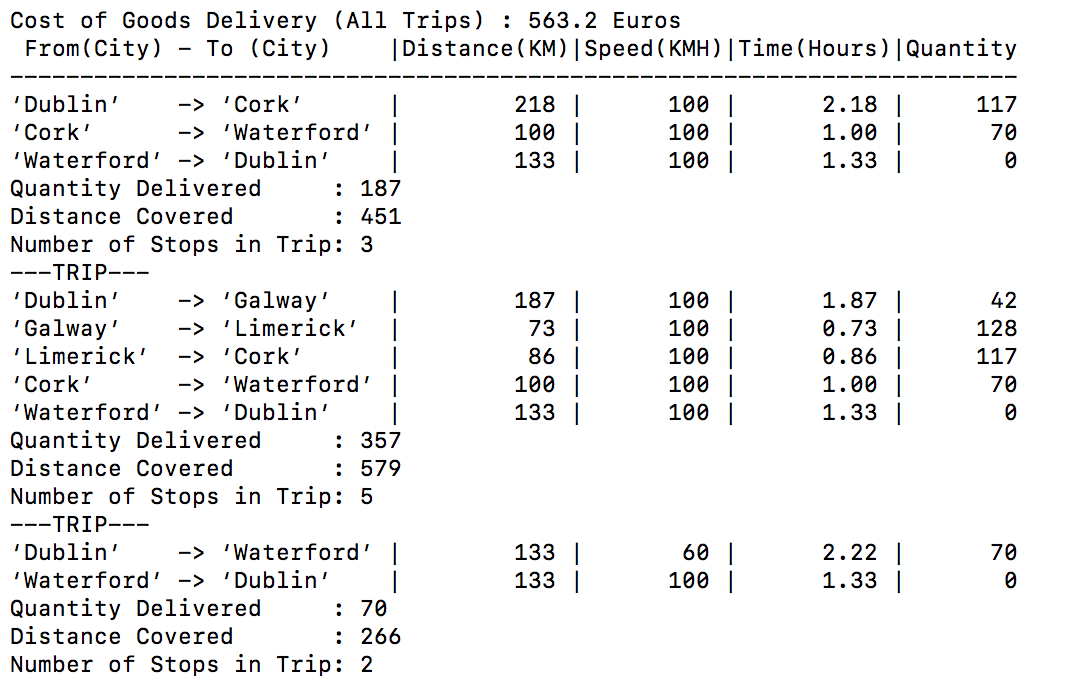
\includegraphics[scale=0.8]{fig1.png}
\begin{figure}[H]
\caption{Goods Delivery Optimal Cost :  With Capacity Constraint - Run1}
\end{figure}
\end{center}


\begin{center}
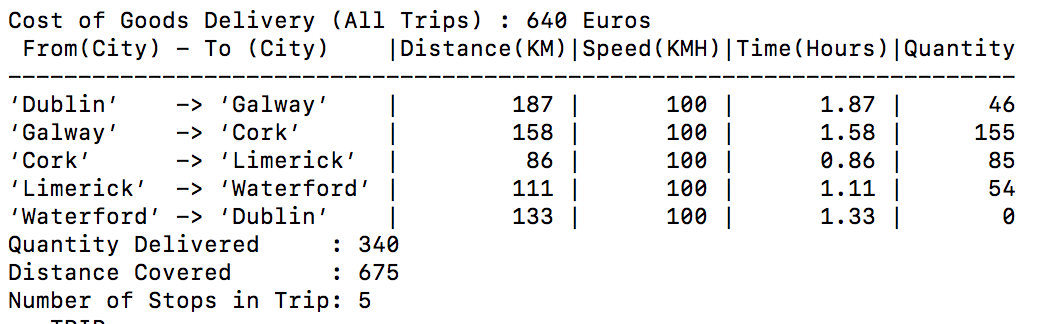
\includegraphics[scale=0.8]{fig2.png}
\begin{figure}[H]
\caption{Goods Delivery Optimal Cost :  With Capacity Constraint - Run2}
\end{figure}
\end{center}

\begin{center}
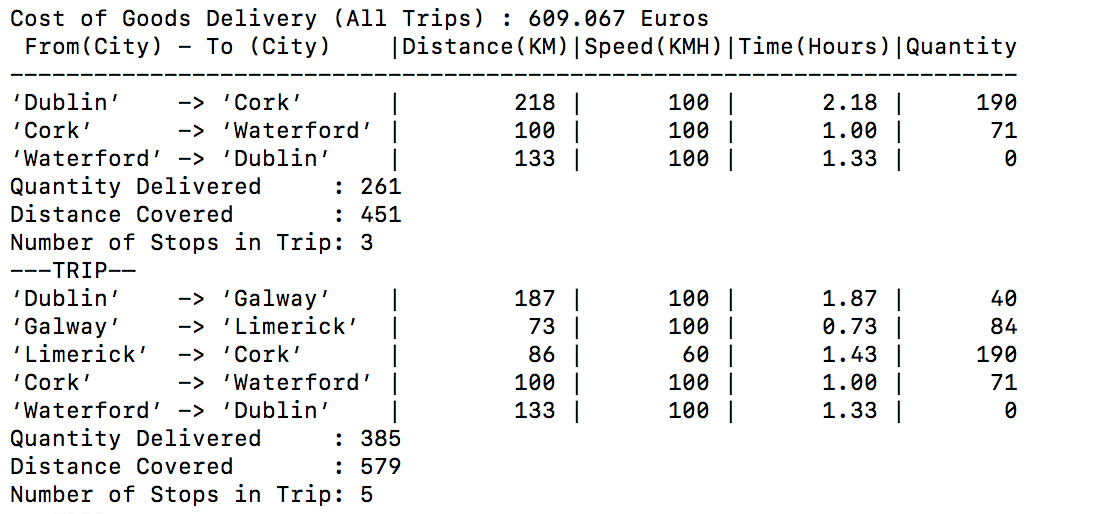
\includegraphics[scale=0.8]{fig3.png}
\begin{figure}[H]
\caption{Goods Delivery Optimal Cost :  With Capacity Constraint - Run3}
\end{figure}
\end{center}

\subsection*{With Capacity Constraint and Time Constraint}

\begin{center}
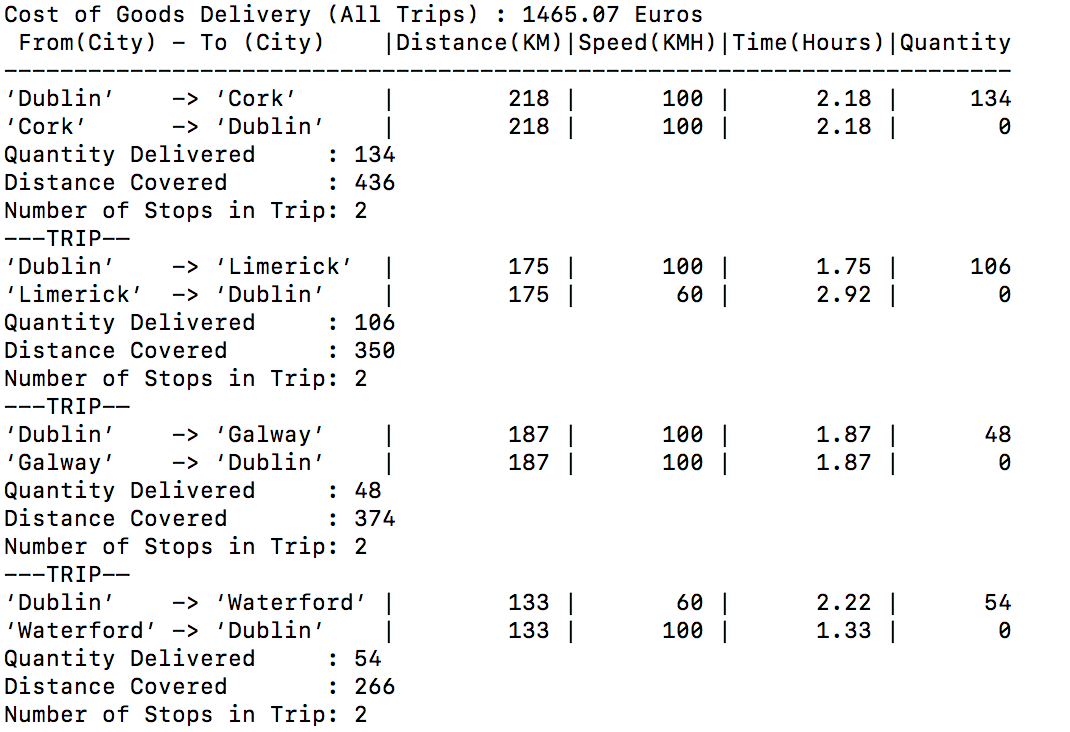
\includegraphics[scale=0.8]{fig4.png}
\begin{figure}[H]
\caption{Goods Delivery Optimal Cost :  With Capacity Constraint  and Time Constraint}
\end{figure}
\end{center}

\section*{Vehicle Routing  - 20 Cities}
\subsection*{With Capacity Constraint and No Time Constraint}

\begin{center}
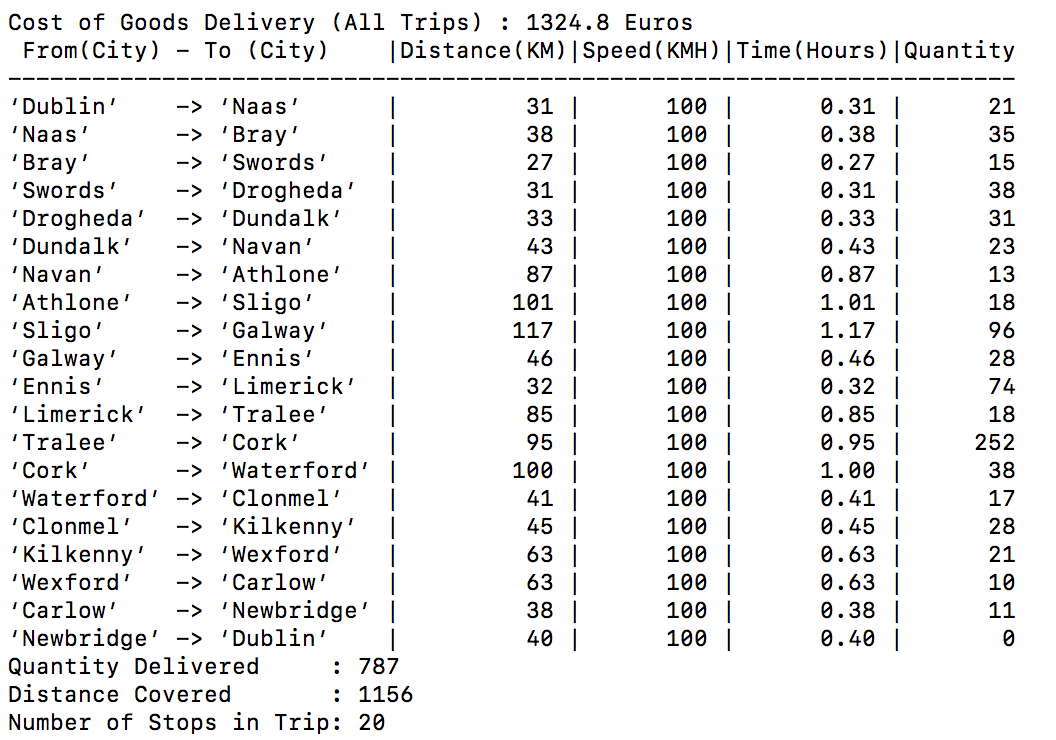
\includegraphics[scale=0.8]{20fig1.png}
\begin{figure}[H]
\caption{Goods Delivery Optimal Cost :  With Capacity Constraint - Run1}
\end{figure}
\end{center}


\begin{center}
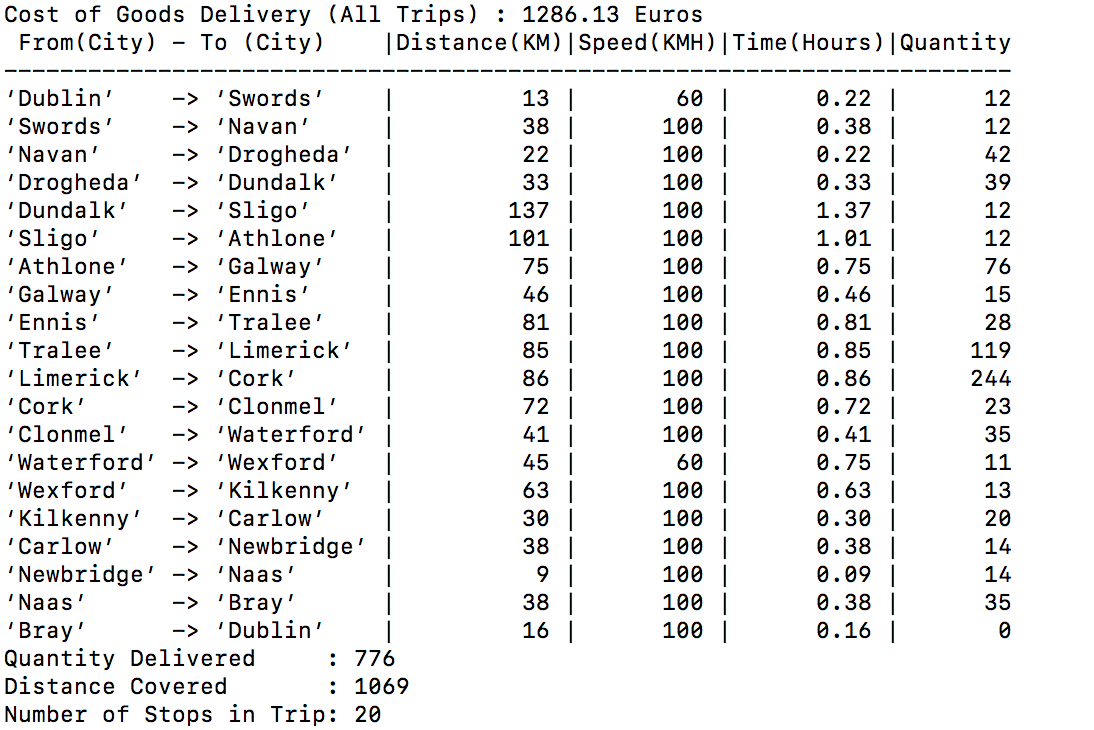
\includegraphics[scale=0.8]{20fig2.png}
\begin{figure}[H]
\caption{Goods Delivery Optimal Cost :  With Capacity Constraint - Run2}
\end{figure}
\end{center}

\begin{center}
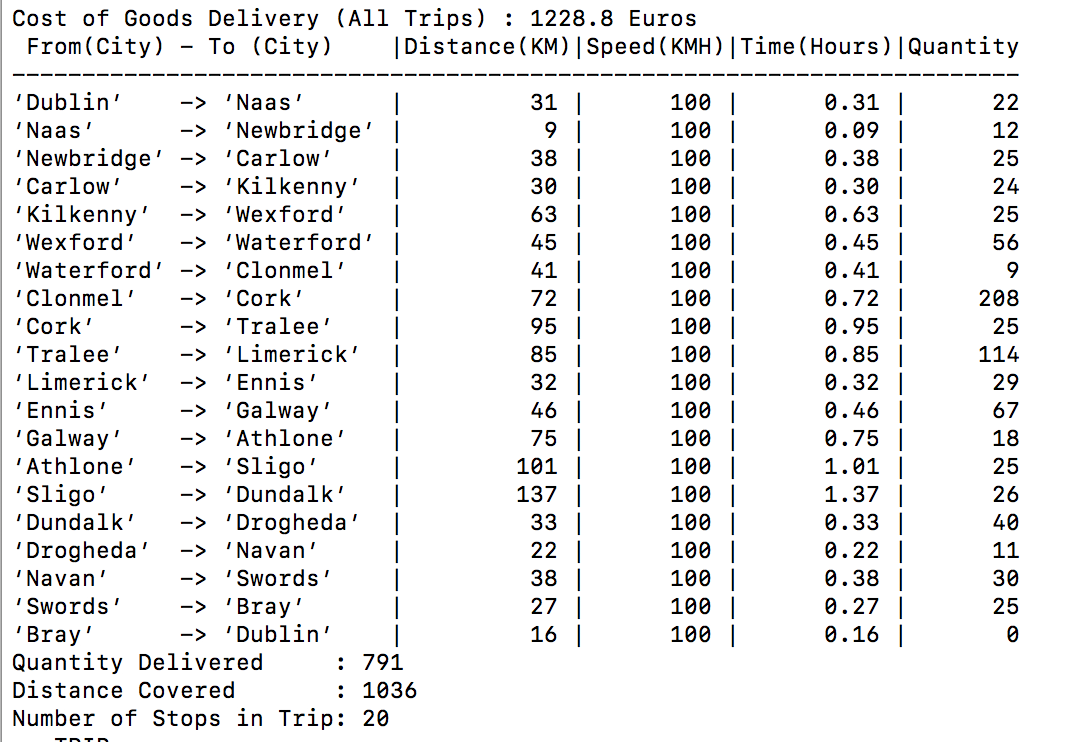
\includegraphics[scale=0.8]{20fig3.png}
\begin{figure}[H]
\caption{Goods Delivery Optimal Cost :  With Capacity Constraint - Run3}
\end{figure}
\end{center}

\subsection*{With Capacity Constraint and Time Constraint}

\begin{center}
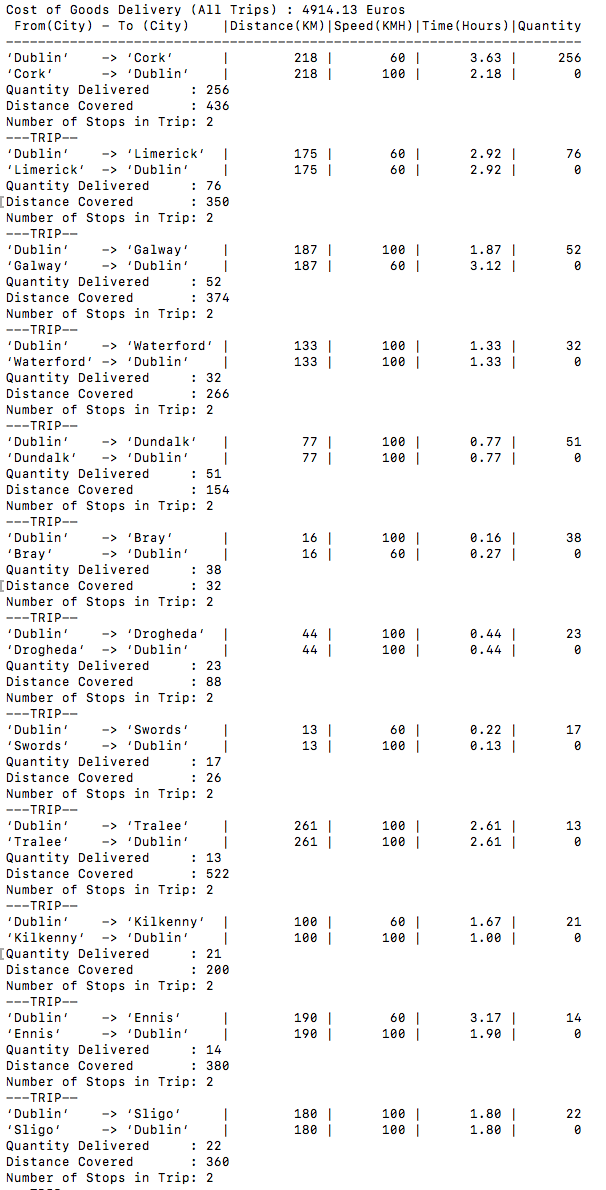
\includegraphics[scale=0.8]{20fig4.png}
\begin{figure}[H]
\caption{Goods Delivery Optimal Cost :  With Capacity Constraint  and Time Constraint}
\end{figure}
\end{center}

\section*{Vehicle Routing  - 30 Cities}
\subsection*{With Capacity Constraint and No Time Constraint}
\begin{center}
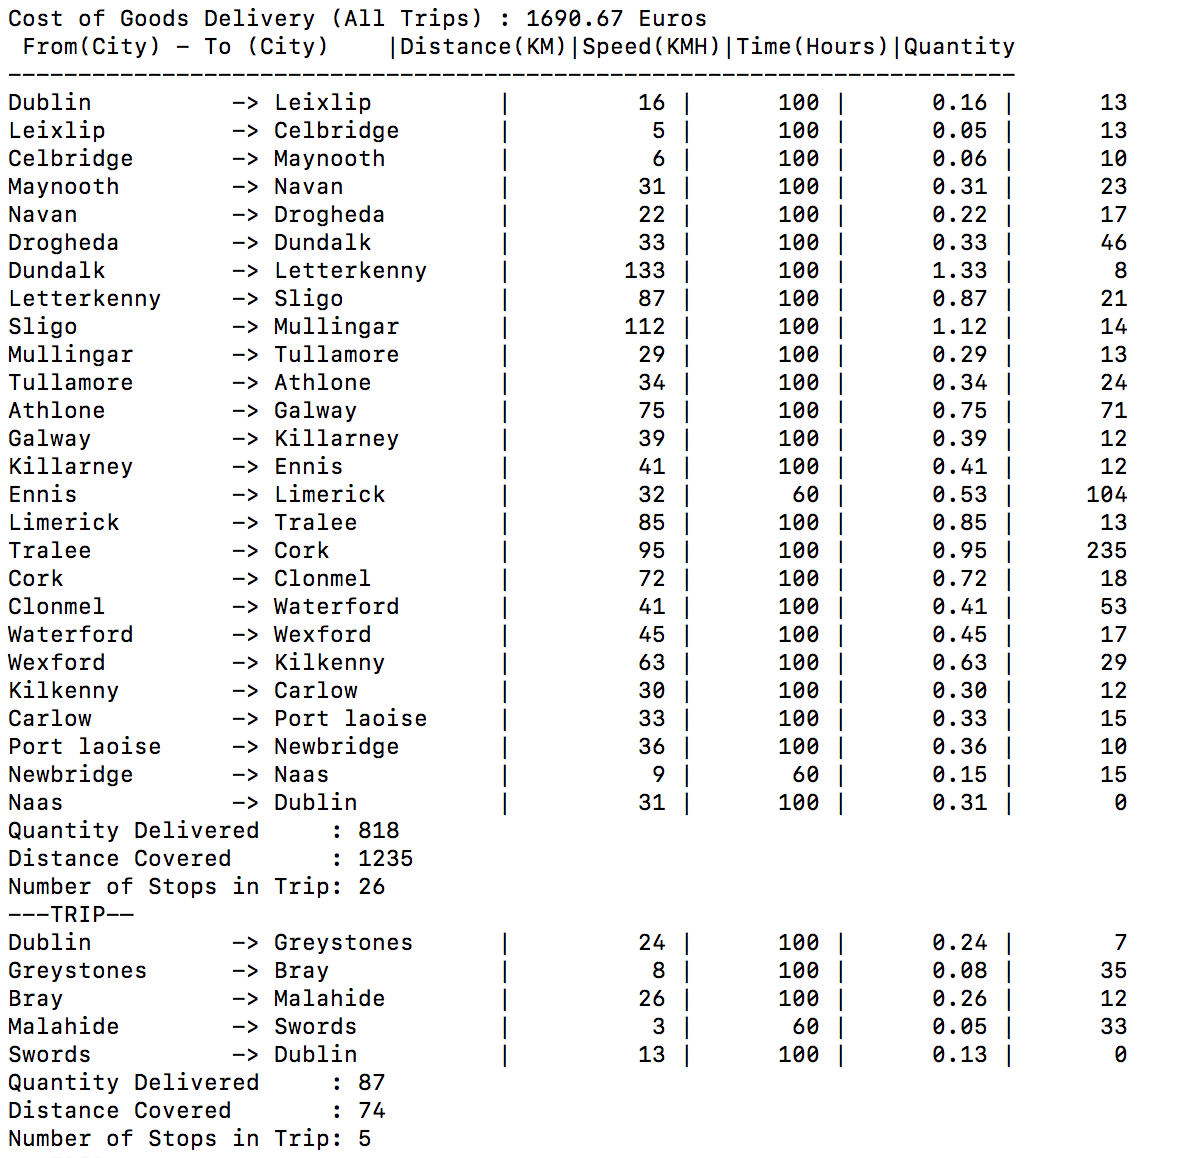
\includegraphics[scale=0.8]{30fig1.png}
\begin{figure}[H]
\caption{Goods Delivery Optimal Cost :  With Capacity Constraint - Run1}
\end{figure}
\end{center}


\begin{center}
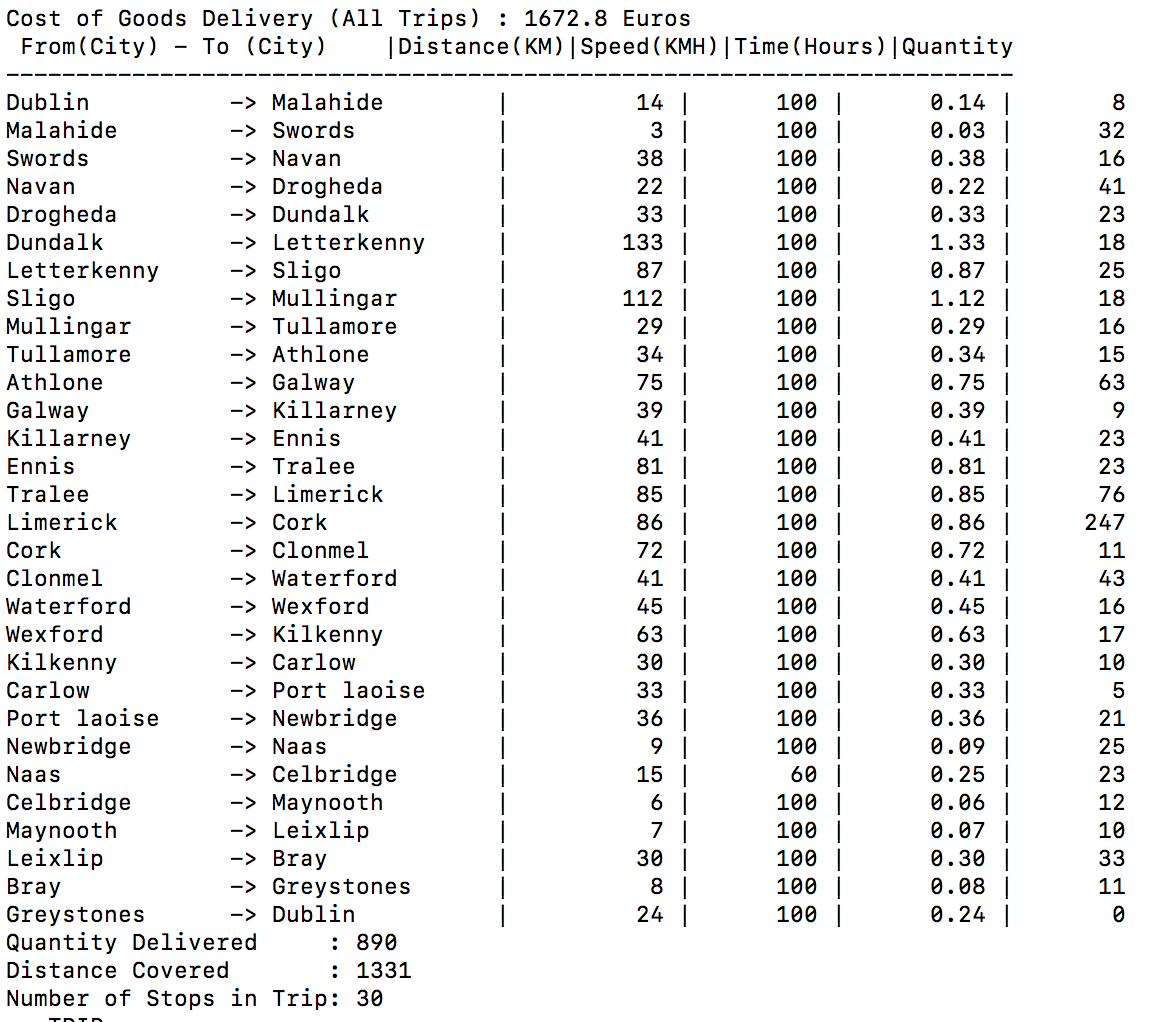
\includegraphics[scale=0.8]{30fig2.png}
\begin{figure}[H]
\caption{Goods Delivery Optimal Cost :  With Capacity Constraint - Run2}
\end{figure}
\end{center}

\begin{center}
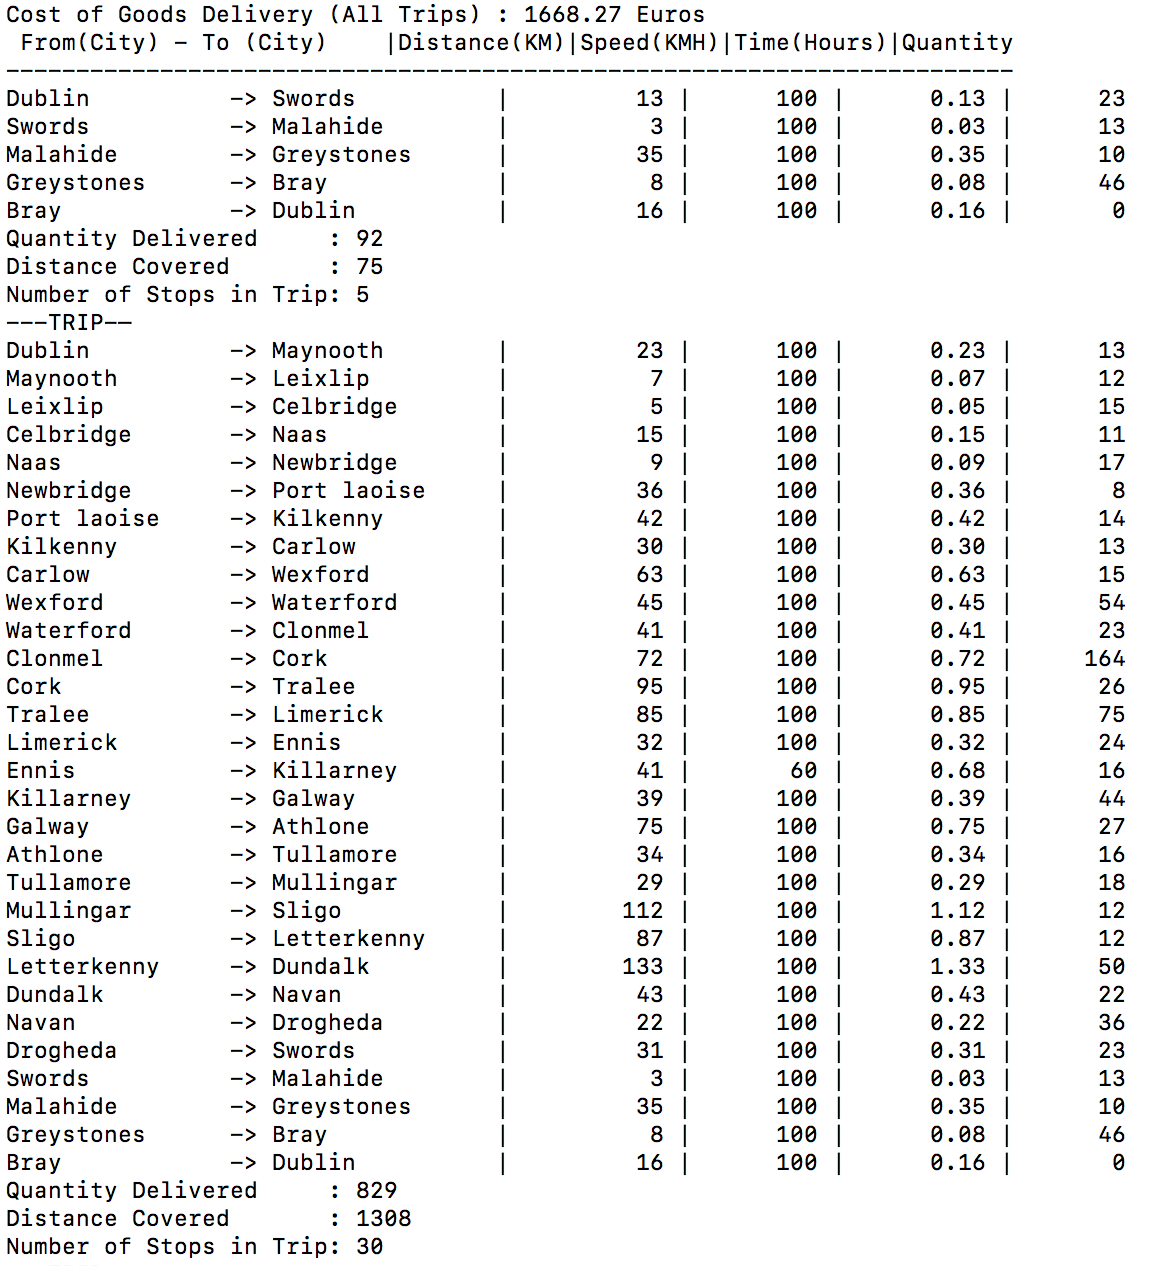
\includegraphics[scale=0.8]{30fig3.png}
\begin{figure}[H]
\caption{Goods Delivery Optimal Cost :  With Capacity Constraint - Run3}
\end{figure}
\end{center}

\subsection*{With Capacity Constraint and Time Constraint}

\begin{center}
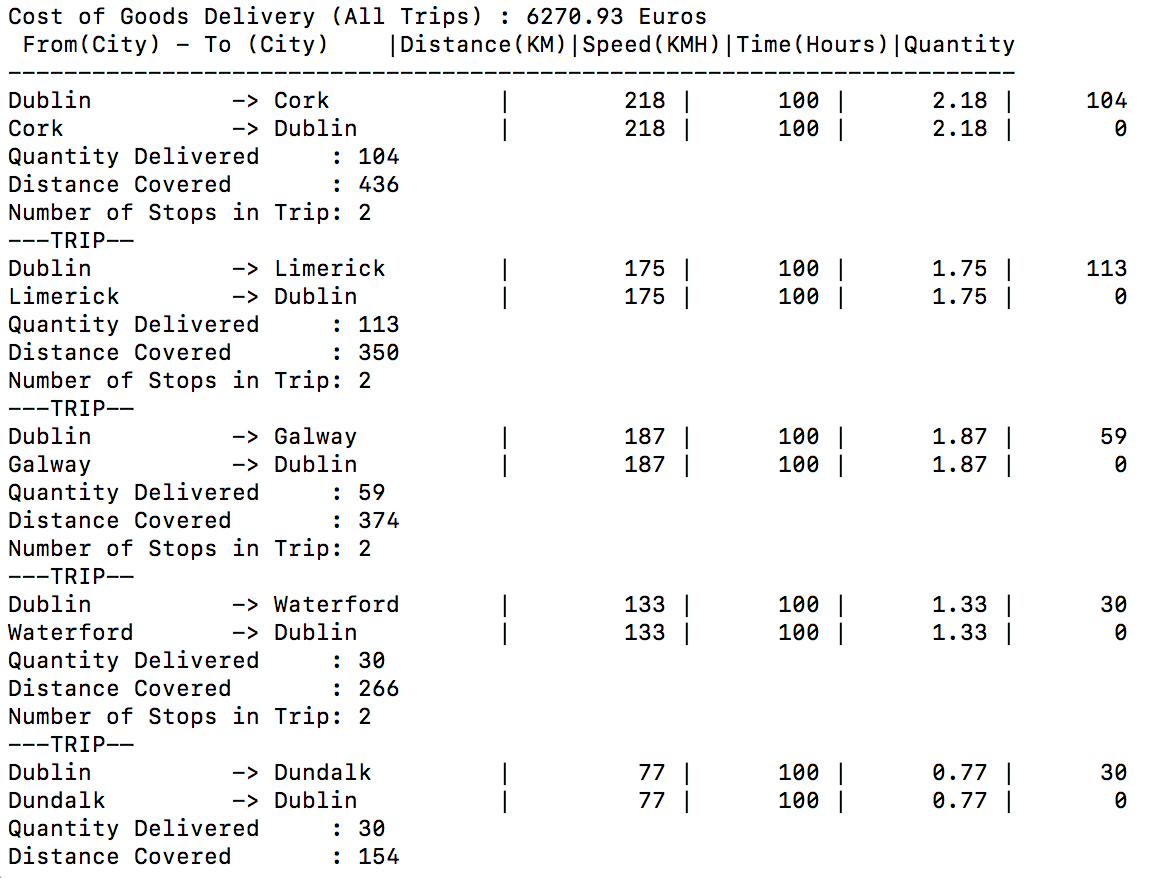
\includegraphics[scale=0.8]{30fig4.png}
\begin{figure}[H]
\caption{Goods Delivery Optimal Cost :  With Capacity Constraint  and Time Constraint}
\end{figure}
\end{center}



\end{document}

\begin{lstlisting}

\end{lstlisting}

\section*{Authorship}

Adedayo Adelowokan Contribution: Started development on the very first Mosel model before the problem was changed, also offered insights into the new Mosel Model. Sections: 1, 3, 7
 \\
\newline
Louis Carnec Contribution: Problem research original and final one, Data Generation in python, 50\% of Mosel Implementation, sections; 2,4,5 \\
\newline
Vijay Katta Contribution: Started research on identifying the problem and changing the original one, 50\% of Mosel implementation, generating the results, sections; 6 \\


\clearpage
\bibliographystyle{acm}
\bibliography{assignment3}

\end{document}